\documentclass[TechnicalNoteMeteo.tex]{subfiles}

\begin{document}

The algorithm described in this paper is based on the implementation of the classical MLR (Multiple Linear Regression) method presented in \cite{eischeid_creating_2000}. The MLR method is a robust and well known spatial interpolation technique that can indirectly account for local effects, such as topography, land cover, land use and surface water. While creating serially complete daily datasets of air temperature and total precipitation for the western U.S., \cite{eischeid_creating_2000} found that the MLR method consistently outperformed the other classical methods tested (normal ratio, inverse distance, optimal interpolation, and single best estimator). The same result was also found by \cite{xia_forest_1999} for a study in Bavaria, Germany. Moreover, in a study conducted in Iran for different climate conditions (dry to extra humid conditions), \cite{kashani_evaluation_2011} found that the estimation obtained with the MLR method compared well with those obtained with more recent methods, more specifically the artificial neural network (reference) and the genetic programming (references) techniques.

\Cref{fig:fillworker_flowchart} presents a flowchart of the algorithm developed for filling the gaps in the daily weather dataset of a given target station using data from the neighboring stations. The algorithm consists of two nested loops: the external `Loop A' iterates over the weather variables in the dataset of the target station (min, max, and mean air temperature and total precipitation), while the inner `Loop B' iterates over the missing values in the data series of a given variable. Each missing value is estimated independently with a two-step procedure. The first step consists in the selection of the neighboring stations. The second step consists in building a MLR model and estimating the missing value in the dataset of the target station. 

\begin{figure}[!p]
    \centering
    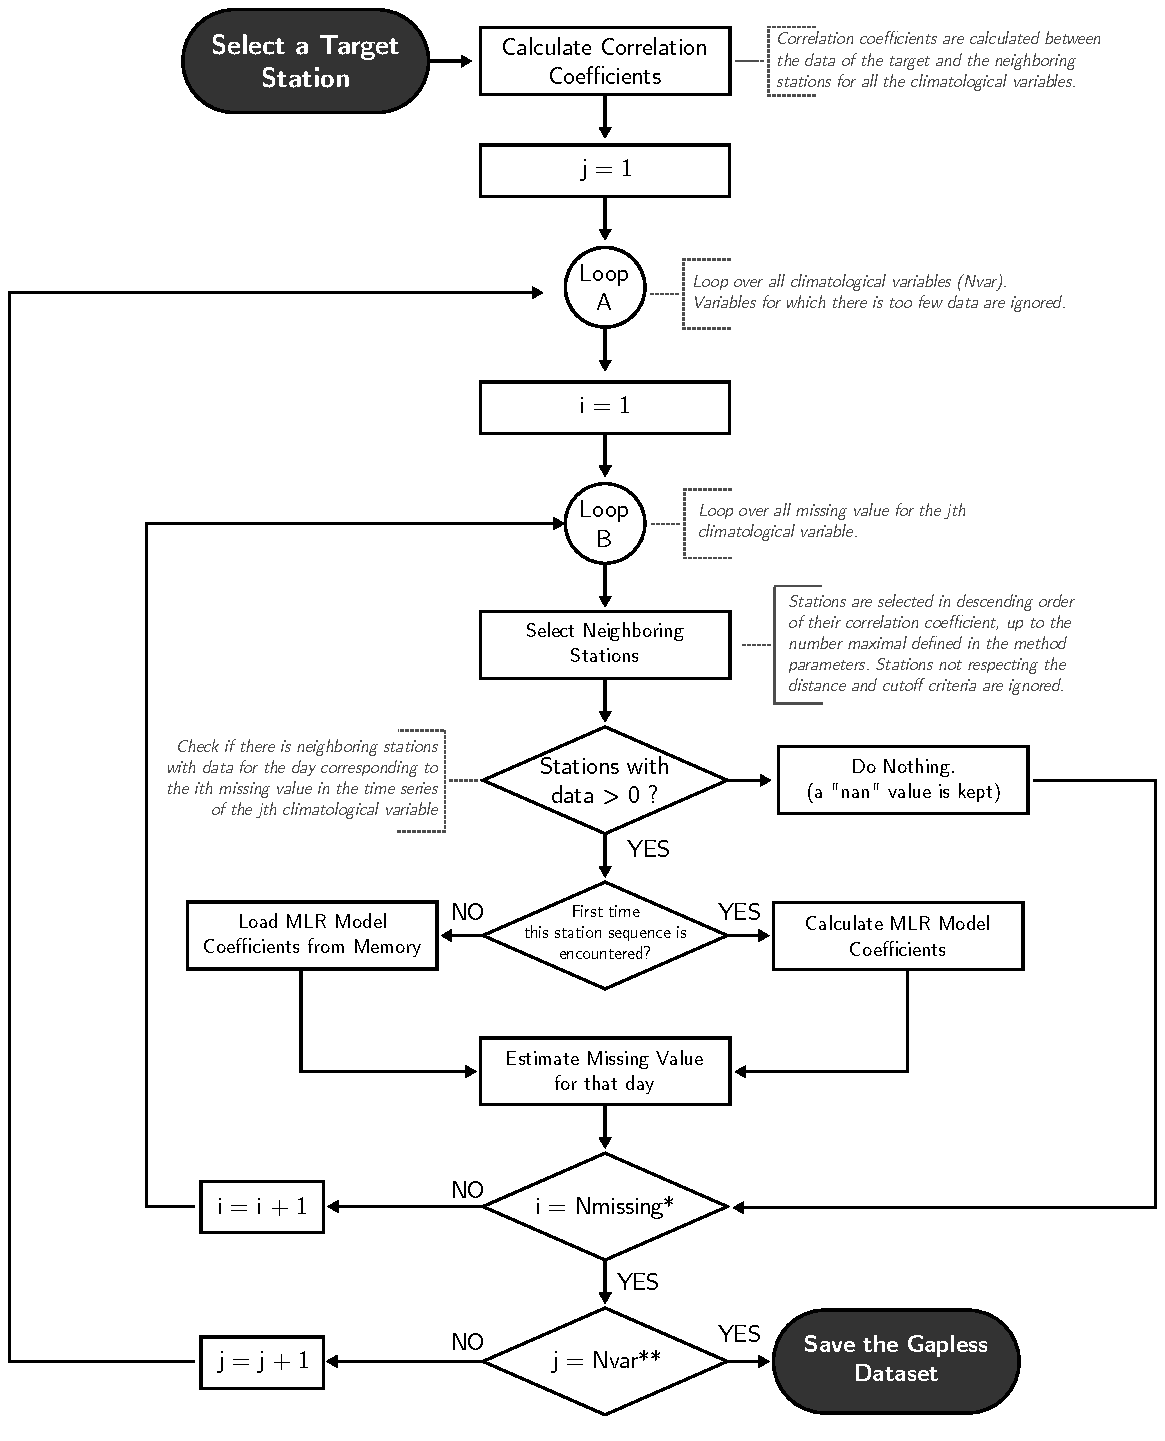
\includegraphics[width=\textwidth]{img/Flowchart-filling_missing_weather.pdf} 
    \caption{}
    \label{fig:fillworker_flowchart}
\end{figure}

\subsection{Loop A}

\subsubsection{Correlation Coefficients Calculations}

The first step consists in calculating the correlation coefficients between the available data of the target station and those of the neighboring stations for the j\textsuperscript{th} weather variable of the dataset. A correlation coefficient is calculated for each neighboring station individually using all the available data. Neighboring stations that have less than 182 days (half a year) with synchronous data with the target station or with a correlation coefficient below a value of 0.35 are discarded and won't be used for filling the gaps the time series of the target station for this weather variable. The 0.35 threshold for the correlation coefficient is based on the value used by \cite{eischeid_creating_2000} in theirs application of the method. 

Moreover, data correlation between two stations will generally decreases as the horizontal and vertical distances between them increase. It is therefore possible to specify a cutoff distance and a cutoff altitude difference for which neighboring stations that fall above these cutoff values are thereafter ignored in the gapfilling algorithm. The default values are set to \SI{100}{km} and \SI{350}{m} for the horizontal and vertical distance respectively based on the literature \cite{tronci_comparison_1986,xia_forest_1999,simolo_improving_2010}.

\subsection{Loop B}

\subsubsection{Selection of the neighboring stations}\label{sec:select_stations}

The selection of surrounding stations is critically important for the accurate estimation of missing weather data \cite{eischeid_creating_2000}. Problems arise though because the list of neighboring stations with available data can vary from one day to the other. Therefore, it is not possible to use a single MLR model to estimate the missing values in the dataset of the target station all at once. The selection of the neighboring stations and the generation of a MLR model must be done instead individually for each missing value in the dataset of the target stations.

Neighboring stations with available data are selected in descending order of their correlation coefficient, up the a maximal number of stations that was set in the method parameters. The default value for the maximal number of neighboring station used for the construction of the MLR models is set to four. Tests run by \cite{eischeid_creating_2000} showed that using more then four stations did not significantly improve or degraded the accuracy of the estimate. If for a given day with a missing value, no neighboring stations have a measured value, no calculation is done and a ‘NaN' value is kept in the dataset. 

\subsubsection{Generation of the Multiple Linear Regression Model}

Each time a MLR model is generated for a given sequence of neighboring stations, the program stores the model parameters into memory. Therefore, after the selection process of the neighboring stations is done for a given day with a missing data (\cref{sec:select_stations}), the program checks if the sequence of selected stations has already been encountered before for the current weather variable. If so, the stored MLR parameters will be use directly to estimate the missing data for the current day. Otherwise, the model will generate a new MLR model and will store the results into memory. Since a MLR model is generated only one time for a given sequence of neighboring stations, this means that the algorithm becomes faster with time.

using either an Ordinary Least Square (OLS) or a Least Absolute Deviations (LAD) criteria (both options are available). Since daily precipitation series generally represented by long-tailed, positively skewed, distributions, the LAD criterion is typically a better option than the OLS criteria for handling this kind of distribution because it is more robust to outliers (Eischeid et al., 2000, 1995). The downside is an increase in computation time. The MLR using a LAD criterion is computed in WHAT with an iterative reweighted least-squares method (Schlossmacher, 1973; (Eischeid et al., 1995).


\subsubsection{Estimating Missing Daily Values}

Once the parameters of the MLR model for a given day with a missing value are known, the missing value in the target time series is estimated as:

\begin{equation}
    X(t) = a_0 + \sum_{i=1}^{N} a_i \cdot Y_i(t)
\end{equation}

where Y(t) is the missing value of the target station estimated at time t, Xi are the synchronous values of the neighboring stations, ai are the regression coefficients and N is the total number of neighboring stations used for the regression, up to the maximal value defined in the method (default is four).

When all missing values in the target station dataset have been estimated, the resulting gapless time series is saved in a `.out' file. Detailed information about the estimated values are saved in an accompanying `.log' file.

\subsection{Step 3: Validation}

WHAT also includes an option to perform a validation of the method used for a particular weather dataset with a cross-validation procedure.

More specifically, when this option is activated, WHAT will estimate a value for the target station for every day of the time series. In other words, loop B in the flowchart of Figure 8.1 will run over all the days of the dataset and not only over days for which there is a missing data. In addition, the memory feature will be deactivated and a MLR model will be estimated for each day independently. If a measured value is present for the current day being estimated, this value will be temporarily discarded from the data series to avoid self-influence of the observation on the estimation procedure

Consequently, the activation of this feature will significantly raise the computation time for filling the gaps in weather time series and should be used only when a detailed analysis of the estimation errors is required. The default information provided in the ‘‘.log’’ should contain sufficient material to fill the needs of a large number of projects. Thus, this process leads to the production of a weather time-series for which every value has been estimated in WHAT. The results are saved in a tsv (tab-separated values) text file with the extension ‘‘.err’’ that is named after the station name and ID similarly to the ‘‘.log’’ and ‘‘.out’’ files.
The accuracy of the estimation technique can then be assessed by comparing the estimated weather data with the respective non-missing observations in the original weather data file. There is currently no tool provided in WHAT to directly analyze the results from the Jackknife procedure. However, all the source code that has been written? for the production of the figures of Section 8.4 can be downloaded freely on GitHub at (https://github.com/jnsebgosselin/WHAT).

\end{document}

%\subsubsection{Quality Control}

%Prior to the analysis of weather time series, it is important to apply quality control constraints to ensure that the data do not violate obvious constraints associated with minimum, maximum, and average daily air temperature and daily cumulative precipitation. 

%The program will identify irregularities or inconsistencies to insure that maximum, minimum and average daily temperatures are coherent for a given day and that all daily precipitation values are positive. Erroneous values are replaced by nan values in the dataset. These values will subsequently be estimated by the program from neighboring stations.

%The first step of the procedure consists in the selection of the neighboring stations, whose data will be used to estimate the missing value in the dataset of the target station. The second step consists in building a MLR model and estimating the missing value.

%Among these techniques, methods based on the use of data from neighboring stations are generally favored to within-station methods, i.e. those that only use data from the series being filled.

%have been proven to perform poorly compared to methods based on the use of data from neighboring stations for the reconstruction of daily precipitation time series (Eischeid et al., 1995; Kemp et al., 1983; Simolo et al., 2010).

%The creation of a serially complete weather dataset generally consists in the replacement of missing daily data with estimated values calculated from simultaneous observations at nearby stations. 

%Numerous spatial interpolation techniques exist for handling the missing data in the weather time series of a given station by using data from irregularly spaced neighboring station (e.g. simple arithmetic averaging, inverse distance method, single best estimator and multiple regression analysis).

% An example of this problem is illustrated in \cref{tab:selectStations}, where theoretical time-series of air temperature data are presented. In this example, there are missing values in the dataset of the target station, Y, for days 2, 4, and 5. Therefore, the missing value on day 2 will be estimated with data from the neighboring stations X1, X3, and X4 since there is also a missing value on this day for station X2. All neighboring stations will be used for the estimation of the missing value on day 4. Finally, only stations X1 and X2 will be used for the estimation of the missing value on day 5.
%
%\begin{table}[!hb]
%\newcommand{\nan}{\multicolumn{1}{c}{\textbf{nan}}}
%\center
%\caption{This table shows some data}
%\begin{tabular}{
%S[table-format = 1]
%*5S[table-format = 2.1]
%}
%\toprule
%& {Target} & \multicolumn{4}{c}{Neighbors} \\
%\cmidrule(lr){3-6}
%{Day} & {Y} & {X1} & {X2} & {X3} & {X4} \\
%\midrule
%%\rowcolor{gray!30}
%1 & 11.0 & 12.0 & 12.0 & 12.5 & 10.0 \\
%2 & \nan & 12.0 & \nan & 13.0 & 12.2 \\
%3 &   7.5 &  8.5 &   8.5 &  8.0 &  8.9 \\
%4 & \nan &  6.0 &   4.5 &  5.0 &  4.4 \\
%5 & \nan &  8.0 &   8.5 & \nan & \nan \\
%\bottomrule
%\end{tabular}
%\label{tab:selectStations}
%\end{table}
